\subsection{Steuerkennlinie}\label{subsec:Steuerkennlinie}
Die Steuerkennlinie beschreibt die Funktion zwischen dem Input, welches ein 1.2-4V-Regelsignal ist, und dem Drehmoment-Sollwert. Bei diesen Messungen geht es darum, diese Funktion zu bestimmen, um später das angelegte Moment am Motor ohne direkte Kraftmessung regeln zu können. Die Versuchsbedingungen sind in nachfolgender Tabelle \ref{tab:Steuerkennlinie} aufgeführt:

\begin{table}[H]
	\centering
	\begin{tabular}{C{4cm} C{4cm} C{3cm}} 
		\multicolumn{3}{c}{\textbf{Versuchsbedingungen}} \\
		{Messgrösse}& {Bedingung} & {Wert}\\ \hline\hline 
		Spannung (DC)   & nachgeregelt &   96 V     \\
		Strom (DC)   & gemessen &   1.6-107 A     \\
		Leistung (AC)   & gemessen &   0-5666 W    \\
		Drehzahl   & konstant &   1200 RPM    \\
		Drehmoment-Sollwert   & variiert &   0-50 Nm    \\
		Motor-Temperatur   & gemessen &   40-100 °C    \\
		Controller-Temperatur   & vernachlässigt &   -    \\
	\end{tabular}
	\caption{Versuchsbedingungen Steuerkennlinie}\label{tab:Steuerkennlinie}
\end{table}

Wie in der Abbildung \ref{fig:Leistung/Steuerkennlinie} ersichtlich ist, lässt sich das Verhältnis zwischen Drehmoment und Regelsignal mit einer quadratischen Funktion beschreiben. Bei diesem Versuch wird die Leistungs-Temperaturabhängigkeit berücksichtigt, wie sie im Unterkapitel \ref{subsec:Leistung/Temperatur} erklärt wurde.

\begin{figure}[H]
	\centering
	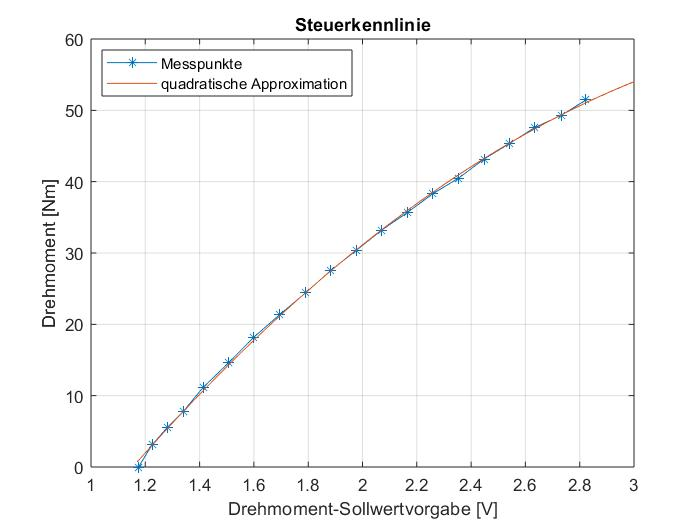
\includegraphics[width=1\linewidth]{Steuerkennlinie.jpg}
	\caption{Steuerkennlinie der Ansteuerung}\label{fig:Leistung/Steuerkennlinie}
\end{figure}

Da der Motor bei diesem Versuch an die thermische Grenze kam und für die geplante Anwendung keine höhere Drehmomente erforderlich sind, wird die Messung nur bis 2.8V durchgeführt. Das Maximum des Drehmoment-Sollwertes liegt jedoch bei 4V.